\documentclass[a4paper,12pt]{article} 

\usepackage[top = 2.5cm, bottom = 2.5cm, left = 2.5cm, right = 2.5cm]{geometry} 

% packages
\usepackage{amsmath, amsfonts, amsthm} % basic math packages
\usepackage{tikz} % for making illustrations
\usetikzlibrary{shapes.arrows, arrows, decorations.markings, positioning}
\usetikzlibrary{calc}
\usetikzlibrary{3d}
\usepackage{graphicx} % for importing images
\usepackage{xcolor} % more color options
\usepackage{colortbl}
\usepackage{multicol} % for making two-column lists
\usepackage{hyperref} % for hyperlinking
%\hypersetup{colorlinks=true, urlcolor=cyan,}
\usepackage{mathabx}
\usepackage{cleveref}
\usepackage{subfig}
\usepackage{array}
\usepackage{wrapfig}
\usepackage{bbm}
\usepackage{fancyhdr}
\usepackage{algorithm, algorithmicx, algpseudocode}
\usepackage{stmaryrd}
\usepackage{physics}


% The following two packages - multirow and booktabs - are needed to create nice looking tables.
\usepackage{multirow} % Multirow is for tables with multiple rows within one cell.
\usepackage{booktabs} % For even nicer tables.

% As we usually want to include some plots (.pdf files) we need a package for that.
\usepackage{graphicx} 

% The default setting of LaTeX is to indent new paragraphs. This is useful for articles. But not really nice for homework problem sets. The following command sets the indent to 0.
\usepackage{setspace}
\setlength{\parindent}{0in}

% Package to place figures where you want them.
\usepackage{float}

% The fancyhdr package let's us create nice headers.
\usepackage{fancyhdr}

% theorems, lemmas, examples, etc.
\newtheorem{theorem}{Theorem}[section]
% \newtheorem{corollary}{Corollary}[theorem]
% \newtheorem{lemma}[theorem]{Lemma}
\newtheorem{example}[theorem]{Example}
\newtheorem{lemma}[theorem]{Lemma}
\theoremstyle{definition}
\newtheorem{definition}{Definition}[section]
\theoremstyle{remark}
\newtheorem*{remark}{Remark}
\newtheorem*{solution}{Solution}

\def\mydefb#1{\expandafter\def\csname bf#1\endcsname{\mathbf{#1}}}
\def\mydefallb#1{\ifx#1\mydefallb\else\mydefb#1\expandafter\mydefallb\fi}
\mydefallb aAbBcCdDeEfFgGhHiIjJkKlLmMnNoOpPqQrRsStTuUvVwWxXyYzZ\mydefallb

\def\mydefb#1{\expandafter\def\csname cal#1\endcsname{\mathcal{#1}}}
\def\mydefallb#1{\ifx#1\mydefallb\else\mydefb#1\expandafter\mydefallb\fi}
\mydefallb aAbBcCdDeEfFgGhHiIjJkKlLmMnNoOpPqQrRsStTuUvVwWxXyYzZ\mydefallb

%% Change this to just the normal N,Z,R,C,P,E
\def\mydefb#1{\expandafter\def\csname bb#1\endcsname{\mathbb{#1}}}
\def\mydefallb#1{\ifx#1\mydefallb\else\mydefb#1\expandafter\mydefallb\fi}
\mydefallb CEGIKNPQRST\mydefallb

\newcommand{\half}{\frac{1}{2}}
\DeclareMathOperator{\sgn}{sgn}
\DeclareMathOperator*{\argmax}{arg\,max}
\DeclareMathOperator*{\argmin}{arg\,min}
\newcommand{\matlab}{\textsc{Matlab}}


%%%%%%%%%%%%%%%%%%%%%%%%%%%%%%%%%%%%%%%%%%%%%%%%
% 3. Header (and Footer)
%%%%%%%%%%%%%%%%%%%%%%%%%%%%%%%%%%%%%%%%%%%%%%%%

% To make our document nice we want a header and number the pages in the footer.

\pagestyle{fancy} % With this command we can customize the header style.

\fancyhf{} % This makes sure we do not have other information in our header or footer.

\lhead{\footnotesize CS 581:  Homework  \# 4}% \lhead puts text in the top left corner. \footnotesize sets our font to a smaller size.

%\rhead works just like \lhead (you can also use \chead)
\rhead{\footnotesize Scott (mtscot4)} %<---- Fill in your lastnames.

% Similar commands work for the footer (\lfoot, \cfoot and \rfoot).
% We want to put our page number in the center.
\cfoot{\footnotesize \thepage} 

\begin{document}
	
	
	%%%%%%%%%%%%%%%%%%%%%%%%%%%%%%%%%%%%%%%%%%%%%%%%
	%%%%%%%%%%%%%%%%%%%%%%%%%%%%%%%%%%%%%%%%%%%%%%%%
	
	%%%%%%%%%%%%%%%%%%%%%%%%%%%%%%%%%%%%%%%%%%%%%%%%
	% Title section of the document
	%%%%%%%%%%%%%%%%%%%%%%%%%%%%%%%%%%%%%%%%%%%%%%%%
	
	% For the title section we want to reproduce the title section of the Problem Set and add your names.
	
	\thispagestyle{empty} % This command disables the header on the first page. 
	
	\begin{tabular}{p{15.5cm}} % This is a simple tabular environment to align your text nicely 
		{\large \sc CS 581:  High Performance Computing} \\
		Emory University \\ Spring 2025 \\ Prof. Tianshi Xu \\
		\hline % \hline produces horizontal lines.
		\\
	\end{tabular} % Our tabular environment ends here.
	
	\vspace*{0.3cm} % Now we want to add some vertical space in between the line and our title.
	
	\begin{center} % Everything within the center environment is centered.
		{\Large \bf Homework \# 4} % <---- Don't forget to put in the right number
		\vspace{2mm}
		
		% YOUR NAMES GO HERE
		{\bf Mitchell Scott}\\ (mtscot4) % <---- Fill in your names here!
		
	\end{center}  
	
	\vspace{0.4cm}
	
	%%%%%%%%%%%%%%%%%%%%%%%%%%%%%%%%%%%%%%%%%%%%%%%%
	%%%%%%%%%%%%%%%%%%%%%%%%%%%%%%%%%%%%%%%%%%%%%%%%
	
	% Up until this point you only have to make minor changes for every week (Number of the homework). Your write up essentially starts here.
	
	\section{Environment}
	
	{\bf List the environment you used to run the code (Operating System, CPU, RAM, etc.). } 
	
	\begin{solution}
		The local environment where I was running the code was on a 2022 MacBook Pro with Apple M2 chip, 8 GB of RAM running macOS Sequoia 15.3.2.  Additionally, my local Apple M2 has 10 built-in GPU cores.
	\end{solution}
	
	\section{Runtime Comparison}
	\textbf{Report the measure outcomes of your two circuits.}
	\begin{solution}
		To ensure that I have correctly coded the quantum teleportation ciorcuit, I have placed the circuit with my \texttt{cirq} circuit in Fig \ref{fig:compare}.
		\begin{figure}[h]
			\centering
			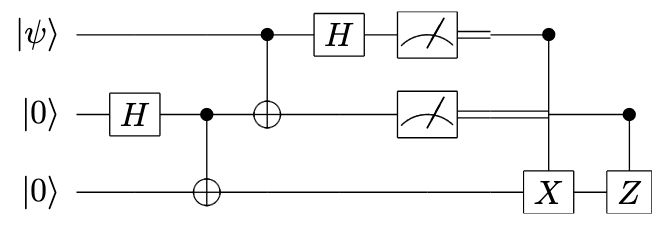
\includegraphics[width=0.40\linewidth]{QTCirc}
			\hspace{1cm}
			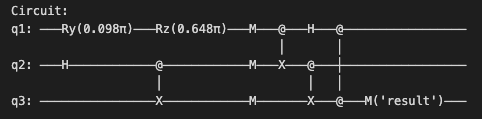
\includegraphics[width=0.40\linewidth]{CirqCirc}
			\caption{\textbf{Left:} The circuit diagram for quantum teleportation as seen in my textbook. \textbf{Right:} The ouputed circuit diagram from my \texttt{cirq} code. }
			\label{fig:compare}
		\end{figure}
		
		Seeing the resemblance between the theoretical gate and the practical gate I created, I knew that my quantum teleportation circuit was correct, so upon running the code to produce the hisogram comparing the number of $\ket{0}, \ket{1}$ in both the randomly constructed quibt and the transported cubit, we see great agreement in Fig. \ref{fig:circuit1}.
		\begin{figure}[h]
			\centering
			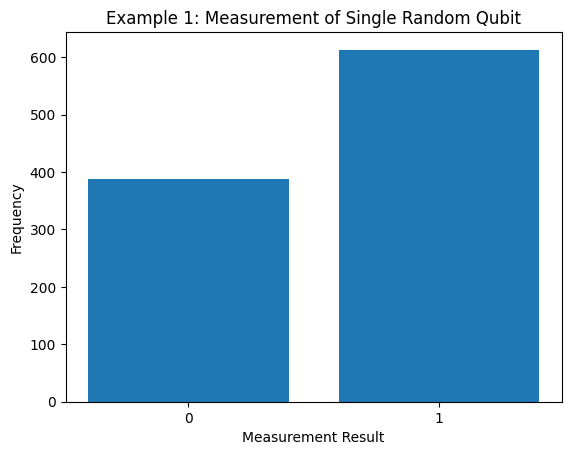
\includegraphics[width=0.45\linewidth]{Circuit1}
			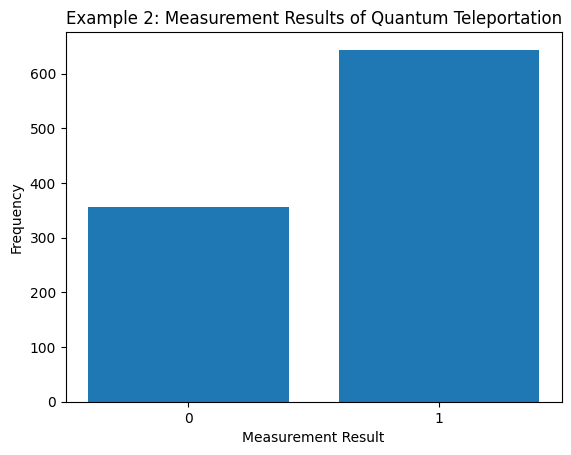
\includegraphics[width=0.45\linewidth]{Circuit2}
			\caption{\textbf{Left:} A historgram displaying the results of measuring the random qubit 1000 times. \textbf{Right:} A histogram displaying the results of measuring the transported qubit 1000 times.}
			\label{fig:circuit1}
		\end{figure}
		Overall, we see similar results, but it is apparent to the naked eye that there is not full agreement. This experiment was run 5 times to see how these results generalize. The random rotation angles in $y$ and $z$ are seen as well as the states and the Hamming distance between the qubit before and after teleportation in Tab. \ref{tab:quantumCounts}. 
		\begin{figure}[h]
			\centering
			\begin{tabular}{|c|c|c|c|c|c|}
				\hline
				Trial &$\bfR_y$&$\bfR_z $ & Alice's $\ket{\phi}$   & Bob's $\ket{\phi}$ & $\norm{\cdot}_{\text{Hamm}}$   \\
				\hline
				1& $0.594\pi$ &$0.011\pi$  &  \{ \textbf{0}: 387, \textbf{1}: 613\}&\{\textbf{0}: 356, \textbf{1}: 644 \}  & 31  \\
				\hline
				2& $0.098\pi$ &$0.648\pi$  &\{\textbf{0}: 969, \textbf{1}: 31\}  & \{\textbf{0}: 972, \textbf{1}: 28\} & 3 \\
				\hline
				3& $0.289\pi$ & $0.69\pi$ & \{\textbf{0}: 819, \textbf{1}: 181\}  & \{\textbf{0}: 818, \textbf{1}: 182\}  &   1 \\
				\hline
				4& $0.825\pi$  & $-0.598\pi$  &\{\textbf{0}: 84, \textbf{1}: 916\}  &  \{\textbf{0}: 90, \textbf{1}: 910\}& 6 \\
				\hline
				5& $0.589\pi$ &$-0.584\pi$  &\{\textbf{0}: 379, \textbf{1}: 621\}  & \{\textbf{0}: 382, \textbf{1}: 618\} & 3 \\
				\hline
			\end{tabular}
			\caption{Running the code 5 times, we observe very similar results in the random qubit and the transported qubit for sundry random rotations, $\bfR_y$ and $\bfR_z$.}
			\label{tab:quantumCounts}
		\end{figure}
		Notice that Trial 1 is the same as the histogram in \ref{fig:circuit1}. However, the results get a lot closer in the other trials, where it appears that there is predominately more of one state compared to the other.
		
		
	\end{solution}
	
	
	\section{Homework Feedback}
	\textbf{Please provide feedback on all four homework assignments if you want (won't be graded). Level of difficulty? Any suggestions?}
	\begin{solution}
		Overall, very nice assignments. Very cool, well thought out, and related to class.
		\textbf{Homework 1:} I think HW1 was a very nice introduction different types of parallel coding like Pthreads and OpenMP.  I think it would also be a fun extension to try to access the data in a column-major way to see how time comparisons can be if you don't use a smart memory access pattern.
		\textbf{Homework 2:} HW2 was tough, but in a very good way. It was really well designed so that we would have to all of them MPI commands. The task of the assignment was very clean. I learned a lot. I wish more assignments were of this caliber.
		\textbf{Homework 3:} I think HW3 was a great and easy introduction to CUDA programming. It was a little on the short side though, and I wish there was another extension, where we had to interact with CUDA code a little more thoroughly.
		\textbf{Homework 4:} Maybe this is juse because I have been doing quantum computing for 5 years now, but this was really simple for me. I also would have liked an assignment on other types of computing like analog computing. 
		\textbf{Beyond Homework 4:} I think it would be really nice for someone who will have to use a lot of parallel code in his life (G-d willing) to have a last homework assignment on matrix algorithms both dense and sparse.
	\end{solution}
	
	
	
	\section*{Acknowledgements}
	I would like to acknowledge that I am done with CS 581: HPC ;P
	
\end{document}
